\section{Appendix}
\subsection{SimpleCNN architectures}\label{codeSnippets}
Initial version of our SimpleCNN, including two convulutional layers:\@

\begin{minted}[mathescape, linenos, fontsize=\scriptsize]{python}
class SimpleCNN(nn.Module):
    def __init__(self, num_classes=10):
        super(SimpleCNN, self).__init__()
        self.conv1 = nn.Sequential(
            nn.Conv2d(
                in_channels = 1,
                out_channels = 32,
                kernel_size = 3,
                stride=1,
                padding="same"
            ),
            nn.LeakyReLU(),
            nn.MaxPool2d(kernel_size=2),
        )
        self.conv2 = nn.Sequential(
            nn.Conv2d(32,64,3,1,"same"),
            nn.LeakyReLU(),
            nn.MaxPool2d(kernel_size=2),
        )
        self.out = nn.Linear(64*7*7, num_classes)

    def forward(self, x):
        x = self.conv1(x)
        x = self.conv2(x)
        x = x.view(-1, 64*7*7)
        output = self.out(x)
        return torch.log_softmax(output, dim=1)
\end{minted}


Structure of the improved version of the SimpleCNN using three convolutional layers, Batch normalization and Dropout:\@

\begin{minted}[mathescape, linenos, fontsize=\scriptsize]{python}
class SimpleCNN(nn.Module):
    def __init__(self, num_classes=10):
        super(SimpleCNN, self).__init__()
        self.conv1 = nn.Sequential(
            nn.Conv2d(1, 32, kernel_size=3, stride=1, padding="same"),
            nn.BatchNorm2d(32),
            nn.ReLU(),
            nn.MaxPool2d(kernel_size=2),
            nn.Dropout(0.25)
        )
        self.conv2 = nn.Sequential(
            nn.Conv2d(32, 64, kernel_size=3, stride=1, padding="same"),
            nn.BatchNorm2d(64),
            nn.ReLU(),
            nn.MaxPool2d(2),
            nn.Dropout(0.25)
        )
        self.conv3 = nn.Sequential(
            nn.Conv2d(64, 128, kernel_size=3, stride=1, padding="same"),
            nn.BatchNorm2d(128),
            nn.ReLU(),
            nn.MaxPool2d(2),
            nn.Dropout(0.25)
        )
        self.fc1 = nn.Linear(128 * 3 * 3, 256)
        self.fc_bn = nn.BatchNorm1d(256)
        self.dropout_fc = nn.Dropout(0.5)
        self.fc2 = nn.Linear(256, num_classes)

    def forward(self, x):
        x = self.conv1(x)
        x = self.conv2(x)
        x = self.conv3(x)
        x = x.view(-1, 128 * 3 * 3)
        x = F.relu(self.fc_bn(self.fc1(x)))
        x = self.dropout_fc(x)
        x = self.fc2(x)
        return torch.log_softmax(x, dim=1)
\end{minted}
    
Structure of the improved version of the SimpleCNN for the PathMNIST dataset:\@

\begin{minted}[mathescape, linenos, fontsize=\scriptsize]{python}
class SimpleCNN(nn.Module):
    def __init__(self, num_classes=10):
        super(SimpleCNN, self).__init__()
        self.conv1 = nn.Sequential(
            nn.Conv2d(3, 32, kernel_size=3, stride=1, padding="same"),
            nn.BatchNorm2d(32),
            nn.ReLU(),
            nn.MaxPool2d(kernel_size=2),
            nn.Dropout(0.25)
        )
        self.conv2 = nn.Sequential(
            nn.Conv2d(32, 64, kernel_size=3, stride=1, padding="same"),
            nn.BatchNorm2d(64),
            nn.ReLU(),
            nn.MaxPool2d(2),
            nn.Dropout(0.25)
        )
        self.conv3 = nn.Sequential(
            nn.Conv2d(64, 128, kernel_size=3, stride=1, padding="same"),
            nn.BatchNorm2d(128),
            nn.ReLU(),
            nn.MaxPool2d(2),
            nn.Dropout(0.25)
        )
        self.fc1 = nn.Linear(128 * 3 * 3, 256)
        self.fc_bn = nn.BatchNorm1d(256)
        self.dropout_fc = nn.Dropout(0.5)
        self.fc2 = nn.Linear(256, num_classes)

    def forward(self, x):
        x = self.conv1(x)
        x = self.conv2(x)
        x = self.conv3(x)
        x = x.view(-1, 128 * 3 * 3)
        x = F.relu(self.fc_bn(self.fc1(x)))
        x = self.dropout_fc(x)
        x = self.fc2(x)
        return torch.log_softmax(x, dim=1)
\end{minted}


\subsection{Data Transformation and Augmentation}\label{training_transformation}

Normalization for ImageNet and Data Augmentation techniques used.

\begin{minted}[mathescape, linenos, fontsize=\scriptsize]{python}
preprocessing = transforms.Compose([
    transforms.Resize(256),
    transforms.CenterCrop(224),
    transforms.ToTensor(),
    transforms.Normalize(mean=[0.485, 0.456, 0.406], std=[0.229, 0.224, 0.225]),
])
 
# augmentations to be applied
augmentations = v2.Compose([
    v2.RandomHorizontalFlip(0.1),
    v2.RandomVerticalFlip(0.1)
])

augmentations_2 = v2.RandomApply(torch.nn.ModuleList(
    [v2.RandomRotation(30),]), p=0.1)
augmentations_3 = v2.RandomApply(torch.nn.ModuleList(
    [transforms.ColorJitter(),]), p=0.1)

\end{minted}

\subsection{WeightedRandomSampler}\label{weightedsampler}
Data balancing with WeightedRandomSampler

\begin{minted}[mathescape, linenos, fontsize=\scriptsize]{python}
    # Calculate weights for each class
    class_weights = [1 / count for count in t_occurences]

    # Create a list of weights corresponding to each sample in the dataset
    sample_weights = [class_weights[int(train_dataset[label_idx][1])] for label_idx in train_set.indices]

    # Convert the list of weights to a PyTorch tensor
    weights = torch.DoubleTensor(sample_weights)

    # Use WeightedRandomSampler to balance the classes
    sampler = WeightedRandomSampler(weights, len(sample_weights), replacement = True) #len(train_set) target_number * num_classes
\end{minted}



\subsection{Pretrained Model Architectures}\label{model_architectures}

\begin{figure}[h]
	\centering
	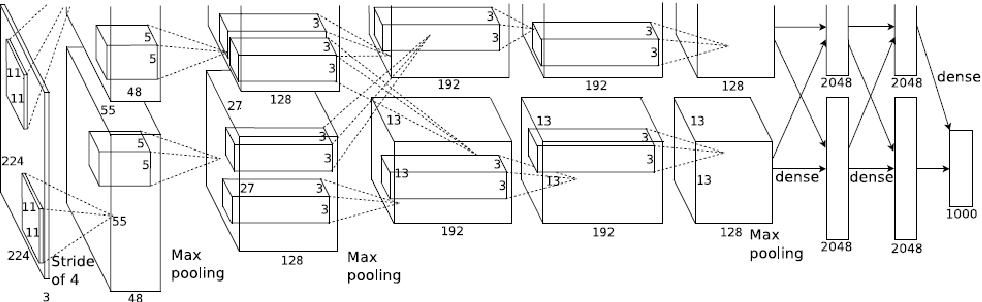
\includegraphics[scale=0.4]{./figures/AlexNet-architecture.png}
	\caption{Original AlexNet architecture given by~\citeauthor{AlexNetoriginal}.}~\label{fig:alexnet}
\end{figure}

\begin{figure}[ht]
    \centering
    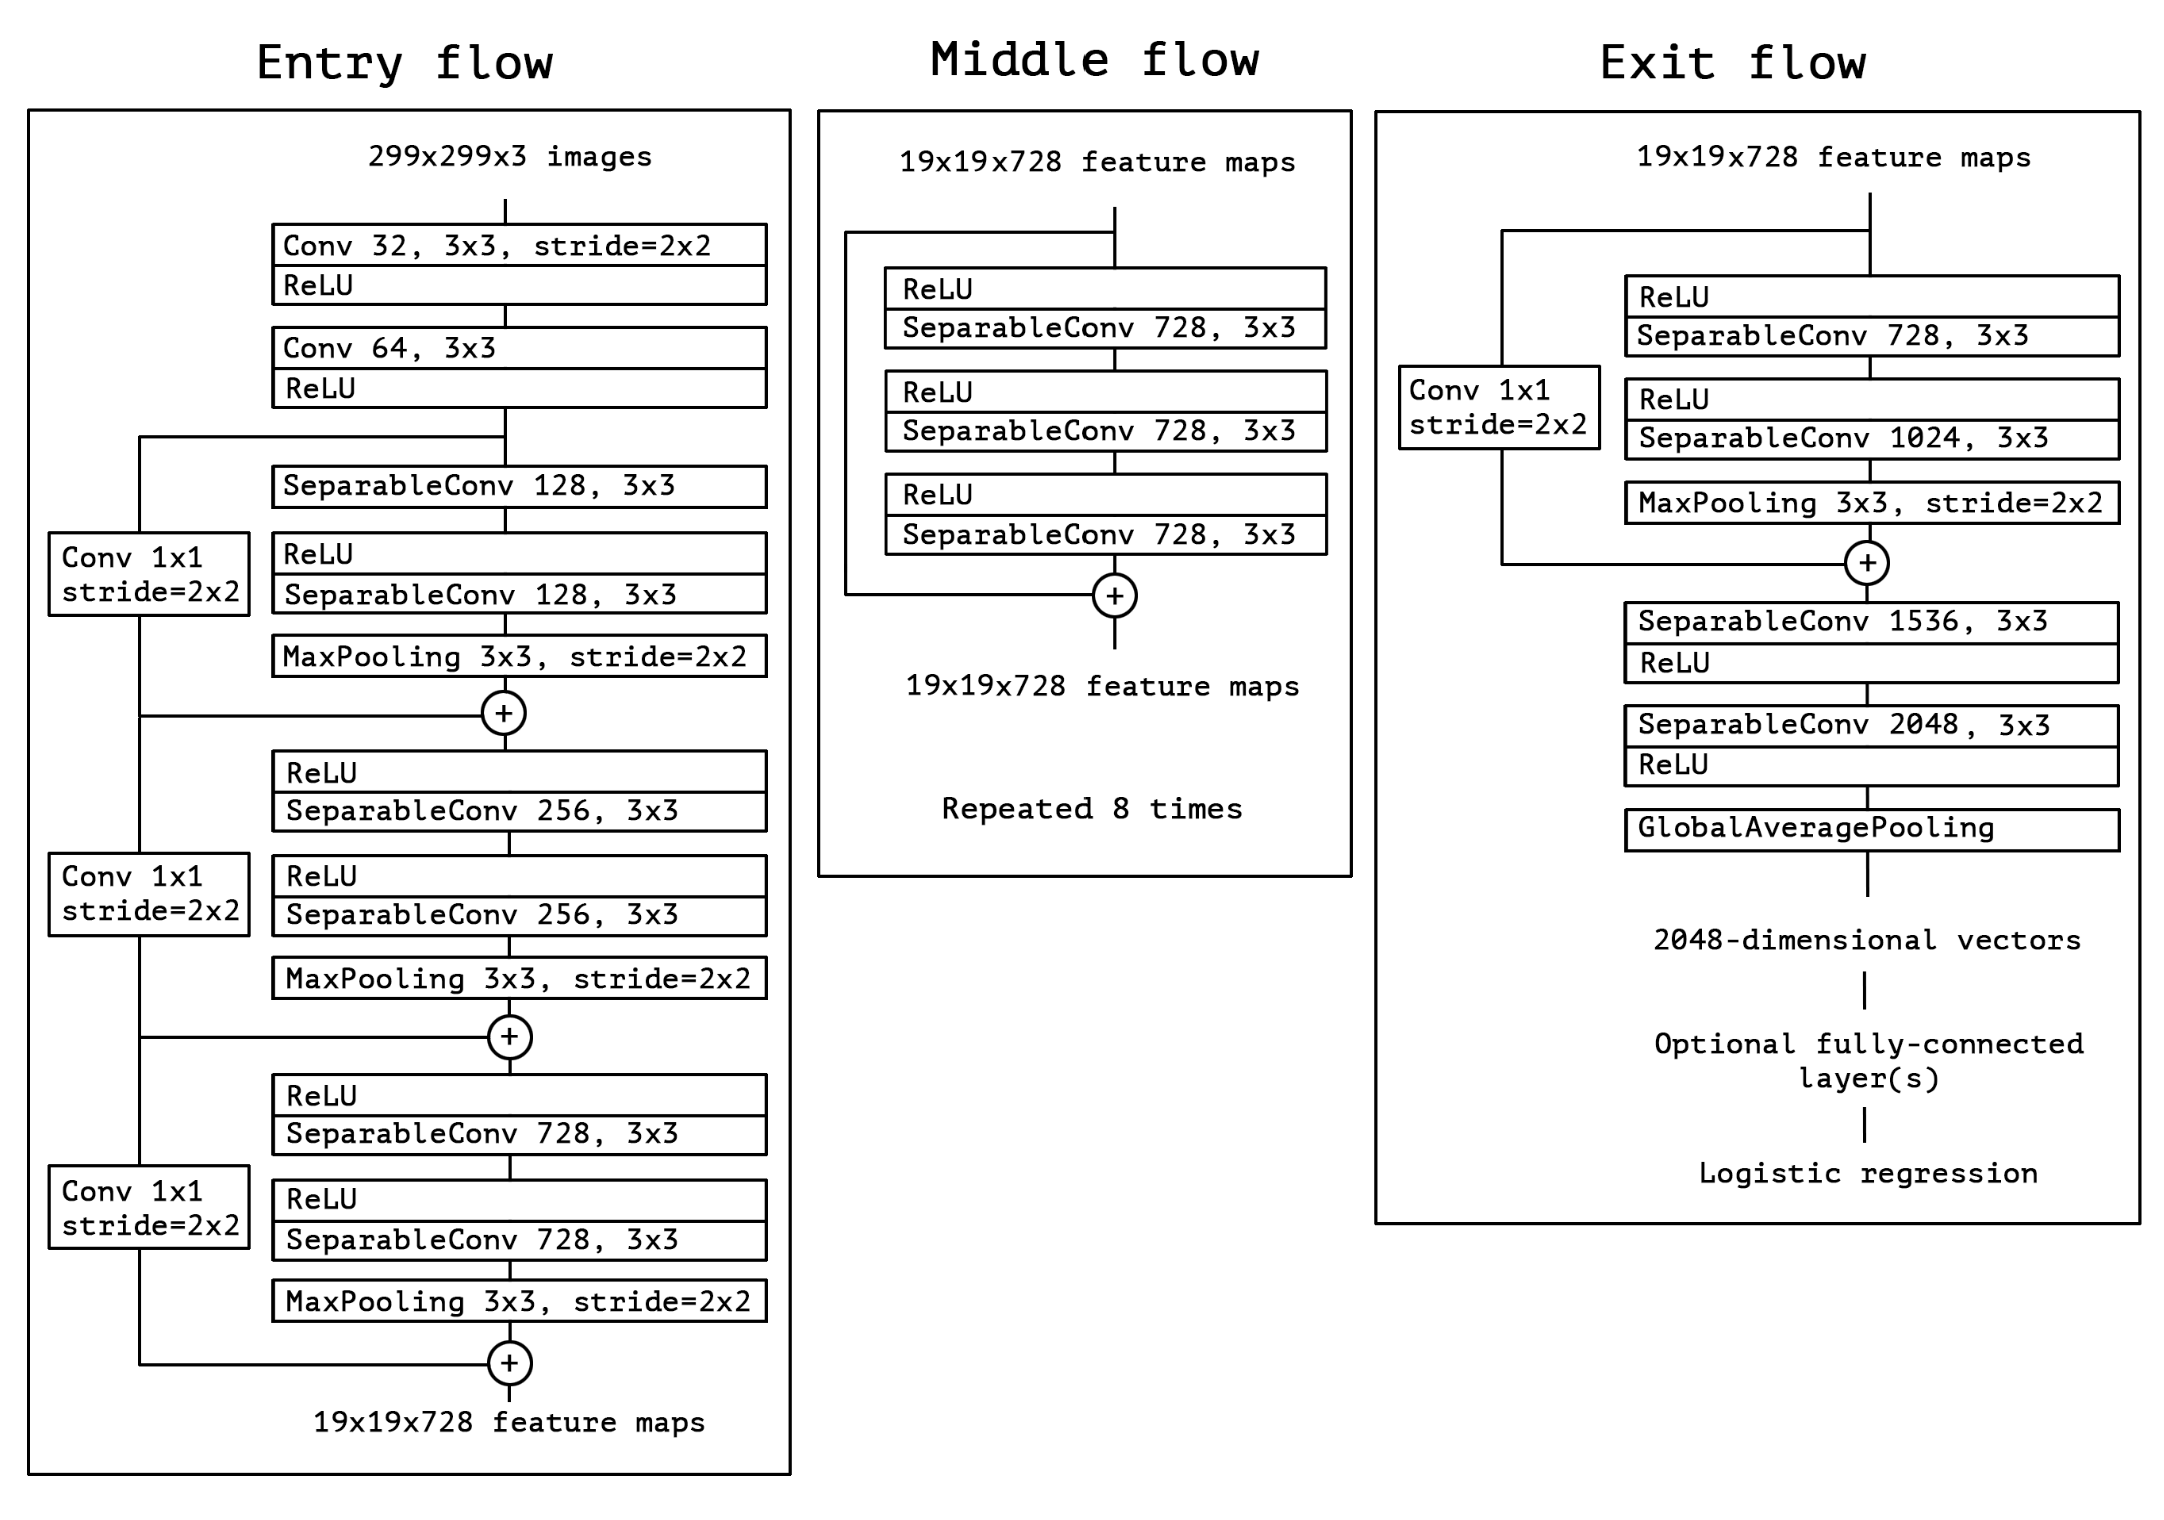
\includegraphics[width=0.9\textwidth]{figures/xception_architecture.png}
    \caption{Xceptions architecture as outlined by \citeauthor{chollet2017xception}.}\label{fig:xceptionArchitecture}
\end{figure}

\subsection{Additional Tables}\label{Appendixtables}

\begin{table}[ht]
    \caption{Impact of Learning Rate, Batch Size, and Epochs on Accuracy in order to determine the best set of Hyperparameters for the SimpleCNN}\label{table:lr_bs_ep}
    \centering
    \begin{tabular}{lll}
    \toprule
    \addlinespace
    \multicolumn{3}{c}{Learning Rate} \\
    \midrule
    Learning Rate & Average Train Accuracy (\%) & Average Validation Accuracy (\%) \\
    \midrule
    0.001 & 99.6 & 98.9 \\
    0.01  & 97.7 & 97.2 \\
    0.1   & 10.3 & 10.0 \\
    \midrule
    \addlinespace
    \addlinespace
    \multicolumn{3}{c}{Batch Size} \\
    \midrule
    Batch Size & Average Train Accuracy (\%) & Average Validation Accuracy (\%) \\
    \midrule
    16 & 99.7 & 98.9 \\
    32 & 99.5 & 98.9 \\
    64 & 99.4 & 98.9 \\
    \midrule
    \addlinespace
    \addlinespace
    \multicolumn{3}{c}{Epochs} \\
    \midrule
    Epochs & Average Train Accuracy (\%) & Average Validation Accuracy (\%) \\
    \midrule
    5  & 99.4 & 98.8 \\
    10 & 99.6 & 99.0 \\
    15 & 99.6 & 99.0 \\
    20 & 99.7 & 99.0 \\
    \bottomrule
    \end{tabular}
    \end{table}